\chapter{Problem}
A pendulum is to be controlled into a vertical orientation on a moving platform.
\begin{figure}[htbp]
        \centering
        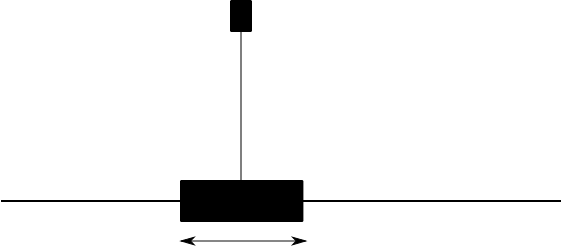
\includegraphics[width=0.95\textwidth]{pendul.png}
        \caption{Pendulum on its moving platform}
        \label{fig:problem}
\end{figure}
The model for this system is:
\begin{equation}
        m\g l \g \Ddot{\theta} + m \g g \g sin(\theta) + k_f \g l \ \dot{\theta} = \frac{T}{l} + \delta_c(t)
\end{equation}

The constants of the system is not precisely known, and can therefore at best be described as:
\begin{equation}
        \begin{split}
                0.095 \leq &m \leq 0.105 \\
                &l = 0.305 \\
                0.4 \leq &k_f \leq 0.6 \\
                &g = 9.81 \\
        \end{split}
\end{equation}

The disturbances from the moving platform is roughly:
\begin{equation}
        \delta_c(t) = 0.0934 \g 5/2000 \g sin(t)
\end{equation}

The goal is to make a sliding mode controller which can hold the pendulum in a vertical orientation, and the speed of the pendulum to be zero; $(\theta, \dot{\theta})= \pi, 0$. The error of the orientation ($\theta$) can at maximum be 0.1 radians to wither side, and the rotation speed ($\dot{\theta}$) can at maximum be 0.01 radians per second.

The controller shall be tested both through simulation and through testing on a real platform.